\chapter{Projet Gestion Recours}
\chapter{Expression des besoins}
\clearpage
\section{introduction}

\subsection{Contexte et présentation du projet}
Les marchés publics au Togo, comme dans de nombreux autres pays, englobent l'ensemble des contrats attribués par les services de l'État (administrations, établissements publics, entreprises publiques et collectivités locales) pour l'acquisition de biens, la réalisation de services et l'exécution de travaux. Cependant, dans le processus de passation ou d’exécution des marchés publics, il peut naître des différends ou litiges, dus à la violation des textes, des clauses contractuelles ou à leur mauvaise interprétation.

Dans un premier temps, toute contestation doit être adressée à l'autorité contractante concernée. Si, après cette démarche, le requérant estime ne pas avoir obtenu satisfaction, il a la possibilité de saisir l'Autorité de Régulation de la Commande Publique (ARCOP) pour un examen approfondi de son recours.

\subsection{Objectifs du projet}
Le projet vise à assurer le suivi et le traitement interne des recours déposés auprès de l'ARCOP, en optimisant leur gestion et en facilitant leur traitement par les différents acteurs impliqués.

\section{Spécifications Fonctionnelles}


\subsection{Filtre des recours}
\begin{itemize}
    \item \textbf{Entre deux dates :} Le logiciel doit permetre de filtrer les recours entres deux dates sur la date de dépot.

    \item \textbf{Par decision :} Le logiciel offrira la possibilité de filter des recours sur les décisions prises .
    \item \textbf{Autres:} Il permettra egalement de filter des recours sur d'autres attributs comme le requérant, l'autorité contractante, etc.

\end{itemize}

\subsection{Enregistrement et mise à jour}
%\begin{itemize}
   L'application doit permettre d'ajouter un nouveau recours et de pouvoir modifier ses informations ultérieurement.
%\end{itemize}
\subsection{Envoi des mails}
%\begin{itemize}
   Cette fonctionalité doit permettre l'envoi automatique de mails, des recours qui tardent à être traités.
%\end{itemize}
\subsection{Vue globale des recours}
\begin{itemize}
   \item Une visualisation graphique du nombre de recours enregistrés en fonction des décisions,
   \item Avec possibilité de filtrer ce graphe entre deux dates.
   \item L'application doit pouvoir afficher les recours en cours de traitement avec leur durée écoulée depuis le dépôt.
\end{itemize}



\section{Spécifications techniques}

\subsubsection{Langages et Technologies}
\begin{itemize}
    \item \textbf{Framework :} Laravel pour une gestion efficace de la logique serveur et du backend.
    \item \textbf{Base de données :} PostgreSQL pour la gestion des données avec Eloquent ORM.
    \item \textbf{Frontend :} Blade pour une interface utilisateur dynamique et fluide.

\end{itemize}


\subsubsection{Sécurité}
\begin{itemize}
    \item Chiffrement des données sensibles.
    \item Gestion des accès par rôles.
\end{itemize}

\subsubsection{Hébergement}
\begin{itemize}
    \item Déploiement sur les serveurs internes de l'\ac{ARCOP}.
\end{itemize}
\subsection{Exigences non fonctionnelles}


\subsubsection{Fiabilité}
\begin{itemize}
    \item Le logiciel doit être disponible 99.9\% du temps, excluant les périodes de maintenance planifiée.
    \item Les données doivent être sauvegardées quotidiennement avec une possibilité de restauration en cas de panne.
\end{itemize}

\subsubsection{Utilisabilité}
\begin{itemize}
    \item L'interface utilisateur doit être intuitive et facile à utiliser, avec une courbe d'apprentissage minimale.
    \item Une documentation utilisateur complète doit être fournie, incluant des guides et des tutoriels.
\end{itemize}

\subsubsection{Compatibilité}
\begin{itemize}
    \item \textbf{Navigateurs :} Le logiciel doit être compatible avec les dernières versions de Chrome, Firefox, Safari, et Edge.
    \item \textbf{Mobile :} L'application web doit être responsive et accessible depuis les navigateurs mobiles.
\end{itemize}

\subsubsection{Scalabilité}
Le logiciel doit pouvoir gérer un nombre croissant d'utilisateurs et de données sans dégradation des performances.


\subsubsection{Nom du logicièl}
Le logiciel sera nommé \textbf{OptiHR}, un nom qui allie modernité et professionnalisme, reflétant une gestion
optimale des ressources humaines.


\section{Définition des acteurs systèmes}
Le logiciel est destiné aux employés de l’\ac{ARCOP} et au département de la Gestion des Ressources Humaines (GRH), facilitant une gestion efficace des congés, de la formation, et des évaluations.
Les utilisateurs principaux du systemes sont:
\begin{itemize}
    \item Employé 
    \item GRH 
    \item DSAF 
    \item DG 
\end{itemize}
\subsection{Employé}
L'utilisateur \textbf{Employé} désignent un employé de l'\ac{ARCOP}. Il utilisent le logiciel pour demander des congés, demander des documents, suivre des formations, et participer aux évaluations. Ils accèdent à leur dossier personnel en ligne pour consulter leur solde de congés, leurs absences, et leurs évaluations.
\subsection{GRH}
Le \textbf{GRH} désigne le \textbf{Chef division des ressources humaines et services généraux} de l'\ac{ARCOP}. Il utilise le logiciel pour gérer les demandes de congés,les documents, les formations, et les évaluations des employés. Il peut consulter les rapports des \ac{RH}, planifier les entretiens,publier des notes ou informations, et suivre les indicateurs de performance.
\subsection{DSAF }
Le \textbf{DSAF} désigne le \textbf{ Directeur des services administratif et financier} de l'\ac{ARCOP}. Il utilise le logiciel pour suivre les demandes effectuées par les employées. IL interagite principallement en consultation.
\subsection{DG}
Le \textbf{DG} désigne le \textbf{Directeur Général} de l'\ac{ARCOP}. Il utilise le logiciel pour valider les demandes de congés, les budgets de formation, et les résultats des évaluations. Il peut consulter les rapports des \ac{RH} et financiers pour prendre des décisions stratégiques en matière de ressources humaines.


\section{D\'efinition des cas d'utilisation}

Un diagramme de cas d'utilisation est une représentation graphique des interactions entre les acteurs d'un système et ses fonctionnalités. Il permet d'identifier et de structurer les besoins fonctionnels du logiciel en décrivant les actions réalisées par chaque acteur. Ce type de diagramme est particulièrement utile pour comprendre les interactions des utilisateurs avec le système et pour définir clairement les responsabilités de chaque acteur.

Dans ce contexte, nous définissons les cas d'utilisation pour chaque fonctionnalités énoncés précédemment.
\subsection{Gestion des recours}
\subsubsection{Description des cas d'utilisation}
\begin{itemize}
    \item \textbf{Enregister un recours :} L'utilisateur peut enregistrer un nouveau recours selon les informations suivantes : le requérant, l'autorité contractante, la date de dépôt et l'objet du recours avec la possibilité de les modifier ultérieurement.
    \item \textbf{Traiter un recours :}Le traitement s'étend de l'étude du recours (aboutissant à une acceptation ou un rejet) jusqu'à une éventuelle décision de fond.
    \item \textbf{Supprimer un recours :} Un recours est supprimable tant qu'il n'est pas encore pris en charge. 
    \item \textbf{Visualiser les recours :} L'utilisateur peut voir tous les recours enregistrés avec les filtres ou afficher les détails d'un recours donné.
   
\end{itemize}
\subsubsection{Diagramme de cas d'utilisation}
\begin{figure}[H]
    \centering
    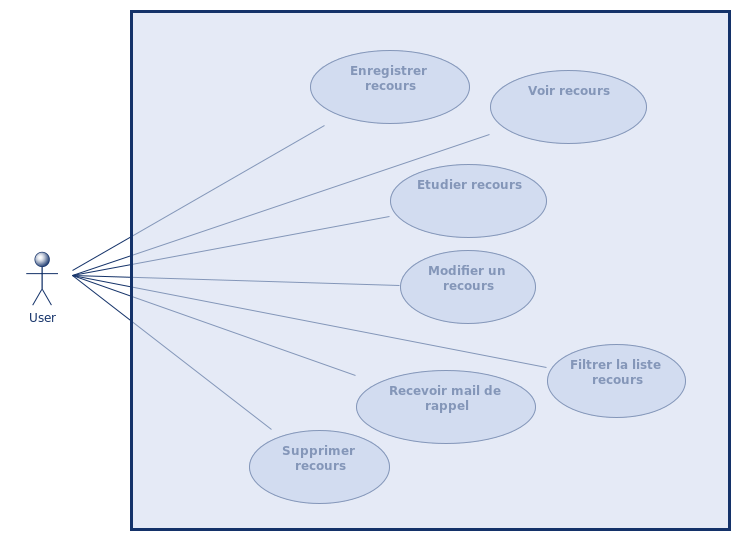
\includegraphics[width=0.8\textwidth]{images/diagrammes/use-cases/Diagramme de cas d'utilisation recours.png}
    \caption{Diagramme de cas d'utilisation Gestion des Recours}
    \label{fig:use_case_gestion_conges}

\end{figure}



\section{Conclusion}
Ce cahier des charges définit les fonctionnalités et les exigences techniques d'un logiciel de gestion des \ac{RH} performant et sécurisé pour l'\ac{ARCOP}. Le logiciel, nommé \textbf{OptiHR}, répondra aux besoins spécifiques du GRH et des employés, en facilitant la gestion des congés, des formations, et des évaluations, d'éditer les bulletins de paie tout en étant évolutif et intégrable aux systèmes existants. La prochaine étape consistera à concevoir l'architecture du système et à élaborer les diagrammes UML pour modéliser les interactions entre les différents modules.
\clearpage
